\chapter{Definición de la empresa}

\section{Descripción de la empresa}

A continuación se presentan los antecedentes institucionales y la identificación formal del establecimiento asistencial de referencia \parencite{hchm2024web}:

\begin{itemize}
    \item \textbf{Nombre:} Hospital Clínico Herminda Martín (HCHM)
    \item \textbf{RUT:} 61.607.001-0 (Establecimiento de salud pública autogestionado en red)
    \item \textbf{Dirección principal (Chillán):} Av. Francisco Ramírez N° 10, Chillán, Región de Ñuble
    \item \textbf{Dependencia institucional:} Servicio de Salud Ñuble, Ministerio de Salud de Chile (MINSAL) \parencite{minsal2022plancancer}
    \item \textbf{Entorno clínico de referencia:} Unidad de Oncología / Centro Ambulatorio de Especialidades (CAE) -- Unidad de Quimioterapia Ambulatoria
    \item \textbf{Dirección del establecimiento:} Dra. Luz María Morán Ibáñez
    \item \textbf{Teléfonos de contacto:} Central telefónica: +56 42 258 6400 | OIRS: +56 42 258 6765
\end{itemize}

\section*{Historia de la empresa}
El Hospital Clínico Herminda Martín de Chillán constituye el principal centro asistencial de alta complejidad y de referencia técnica para la Región de Ñuble. Su origen se remonta al período comprendido entre 1941 y 1945, originado tras el terremoto de 1939 que destruyó el antiguo Hospital San Juan de Dios. La edificación del recinto hospitalario fue posible gracias a la donación testamentaria de doña Herminda Martín Mieres, benefactora que legó los recursos financieros destinados a dotar a la provincia de un moderno establecimiento de salud \parencite{hchm2024web}.

A lo largo de su historia asistencial, el recinto expandió sistemáticamente sus dependencias y cartera de servicios. En la década de 1970 se habilitó el Consultorio Adosado de Especialidades (CAE) y, en la década de 1990, se integraron la Unidad de Paciente Crítico (UPC) y la actual Unidad de Emergencia. Posterior a los daños estructurales provocados por el terremoto de febrero de 2010, el hospital completó un plan integral de normalización y reconstrucción que restituyó su operatividad bajo estándares sismorresistentes \parencite{hchm2024web}.

En el ámbito oncológico, el HCHM consolidó la Unidad de Quimioterapia Ambulatoria dentro del Servicio de Oncología, estableciéndose como el nodo operativo central para la infusión y control de tratamientos sistémicos antineoplásicos e inmunoterapias dirigidos a la población de las 21 comunas que integran la Región de Ñuble \parencite{minsal2022plancancer}.

\section*{Misión}
«Ofrecer una atención integral y de calidad, que contribuye a la recuperación de la salud de las personas, trabajando en equipo, comprometidos e integrados a la red asistencial» \parencite{hchm2024web}.

\section*{Visión}
«Ser un hospital clínico, líder en innovación, para satisfacer las necesidades de salud y elevar la calidad de vida de la comunidad, en forma participativa e inclusiva; con el compromiso de sus trabajadores» \parencite{hchm2024web}.

\section*{Descripción del área de estudio}
El presente proyecto se focalizó exclusivamente en la \textbf{Unidad de Quimioterapia Ambulatoria}, unidad funcional adscrita al Servicio de Oncología y al Centro Ambulatorio de Especialidades (CAE) del Hospital Clínico Herminda Martín. Dicha dependencia concentra los procedimientos de administración parenteral de esquemas citostáticos, terapias biológicas dirigidas y el seguimiento de toxicidades farmacológicas en pacientes oncológicos adultos.

La dinámica operativa de esta unidad presenta una modalidad ambulatoria: el paciente concurre a su sesión de infusión citotóxica en el recinto hospitalario y posteriormente retorna a su domicilio para cursar el período inter-ciclo (comprendido habitualmente entre 14 y 28 días). Durante este lapso domiciliario, el monitoreo y reporte de complicaciones recaen de manera autónoma en el propio paciente o en su cuidador informal.

Por consideraciones asistenciales y de alcance técnico, el área de radioterapia fue excluida del proyecto por dos razones determinantes:
\begin{enumerate}
    \item \textbf{Carencia de infraestructura local y derivación a la macrored:} El Hospital Clínico Herminda Martín no cuenta con equipamiento ni búnker de radioterapia en sus instalaciones de Chillán. Como se constató en las entrevistas al equipo clínico, los pacientes que requieren radioterapia o exámenes de alta complejidad deben ser derivados a prestadores de compra o a centros de la macrored asistencial en la ciudad de Concepción. Por el contrario, la quimioterapia se prepara, administra y controla íntegramente en las dependencias del HCHM.
    \item \textbf{Diferencia en el patrón de toxicidad:} Las complicaciones de la radioterapia corresponden a cuadros loco-regionales con dinámicas asistenciales distintas, mientras que la quimioterapia sistémica induce toxicidades agudas, fluctuaciones hematológicas severas (nadir) y riesgo de descompensación inter-ciclo diario que demandaron un motor de seguimiento continuo y triaje perimetral \parencite{minsal2022plancancer}.
\end{enumerate}

\section{Descripción del problema}
Durante el levantamiento de requerimientos y la observación en terreno en la Unidad de Quimioterapia del HCHM, se evidenció una brecha operacional crítica entre el egreso de la sala de infusión y el reingreso al siguiente ciclo de tratamiento. Como manifestó el personal clínico durante las sesiones de levantamiento técnico: \textit{«nosotros trabajamos muy estrictamente porque los sistemas no nos ayudan»} \parencite{entrevistaHCHM2026}.

El análisis del flujo asistencial reveló factores determinantes que fundamentaron la necesidad de desarrollar una solución tecnológica desacoplada y centrada en el paciente:

\begin{enumerate}
    \item \textbf{Brecha de alfabetización en salud y sobrecarga cognitiva:} En los talleres de inducción a la quimioterapia se identificó que los pacientes enfrentan una barrera importante en la comprensión de su patología y del tratamiento médico, señalando el equipo de salud:
    \begin{quote}
        \textit{«Cuando nosotros vamos al taller de ingreso, los pacientes no saben ni qué es el cáncer... No saben que son células, no saben que proliferan, no saben nada de eso... De tratamiento tampoco saben, no saben qué [es] adyuvante, les dicen: usted va a hacer una quimioterapia neoadyuvante, claro, le hablan en chino [...], pero no le dicen que es una quimio que es antes de la cirugía y con qué propósito está esa quimioterapia»} \parencite{entrevistaHCHM2026}.
    \end{quote}
    Este déficit educativo basal, sumado al impacto del deterioro cognitivo transitorio y fatiga oncológica inducida por fármacos, exigió descartar interfaces complejas en favor de un diseño accesible guiado por la heurística de tres pasos de interacción:
    \begin{quote}
        \textit{«Tenía los 3 clic y eso es lo que tiene que visualizar, los 3 clic son 3 clic que hace para llegar a lo que quiere buscar [...] la gracia es que sea lo más fácil posible, lo más amigable posible, porque [...] si ya no saben de parte de lo que es el cáncer, quizás lo más probable es que tampoco manejen tanto la tecnología. Por eso hay que hacerlo simple nomás»} \parencite{entrevistaHCHM2026}.
    \end{quote}
    Este principio de reducción de costo cognitivo responde a las directrices de usabilidad y accesibilidad priorizadas directamente por el equipo asistencial durante el levantamiento técnico en terreno \parencite{entrevistaHCHM2026}.

    \item \textbf{Dispersión geográfica y brecha de conectividad digital:} De acuerdo con los antecedentes del Censo Oficial y el Plan Nacional de Cáncer, la Región de Ñuble presenta una de las tasas de ruralidad más altas del país junto con los menores niveles de ingreso autónomo \parencite{ine2024censo, minsal2022plancancer}. Gran parte de los pacientes atendidos provienen de sectores rurales con cobertura móvil deficiente o nula. Ante complicaciones críticas como la neutropenia febril (temperatura axilar $\ge 38,0^\circ\text{C}$) en los días de nadir hematológico (días 7 a 14 post-infusión), depender de conectividad continua a servidores en la nube representó un riesgo vital severo \parencite{minsal2022plancancer}.

    \item \textbf{Restricciones clínicas en modelos conversacionales y resguardo de datos:} El equipo clínico enfatizó que la interacción digital debe resguardar estrictamente la privacidad de los datos sensibles y restringir el uso de modelos generativos abiertos que puedan desorientar al usuario:
    \begin{quote}
        \textit{«Primero súper resguardando los datos y lo otro que tampoco promueva, ponte tú, porque acá qué puede pasar que el paciente [...] tenga sintomatología depresiva por la condición en sí. Entonces puede decir me siento mal, no sé qué quiero hacer tal cosa y si la cuestión le afirma, le refuerza más la situación, entonces eso tenemos que evitarlo completamente [...] Y tú crees que los modelos en el fondo siempre como que te dan la razón. Entonces eso igual es un riesgo»} \parencite{entrevistaHCHM2026}.
    \end{quote}
    Esto fundamentó la implementación de un motor de triaje determinista local (\textit{edge computing}) basado en árboles de decisión clínicos cerrados y cuestionarios estructurados condicionales \parencite{entrevistaHCHM2026}, independiente de servicios de procesamiento de lenguaje en la nube para la evaluación de urgencias.

    \item \textbf{Sobrecarga de datos no estructurados y latencia en la toma de decisión médica:} Durante el levantamiento de requerimientos en terreno, se constató que el personal asistencial carecía de mecanismos automatizados para sintetizar los eventos clínicos acumulados durante el período inter-ciclo \parencite{entrevistaHCHM2026}. La revisión manual de registros extensos con predominio de mediciones fisiológicas dentro de rangos normales representaba una sobrecarga informativa inoperativa para el tiempo acotado de la consulta médica. Por ello, el equipo de salud planteó la necesidad crítica de contar con una herramienta de reportabilidad clínica orientada a jerarquizar y filtrar de forma inmediata exclusivamente las variables alteradas y signos de alerta, suprimiendo la dependencia de relatos orales retrospectivos e imprecisos durante la reevaluación del paciente \parencite{entrevistaHCHM2026}.
\end{enumerate}

\newpage
\begin{landscape}
\thispagestyle{empty}

\vspace*{\fill}
\centering
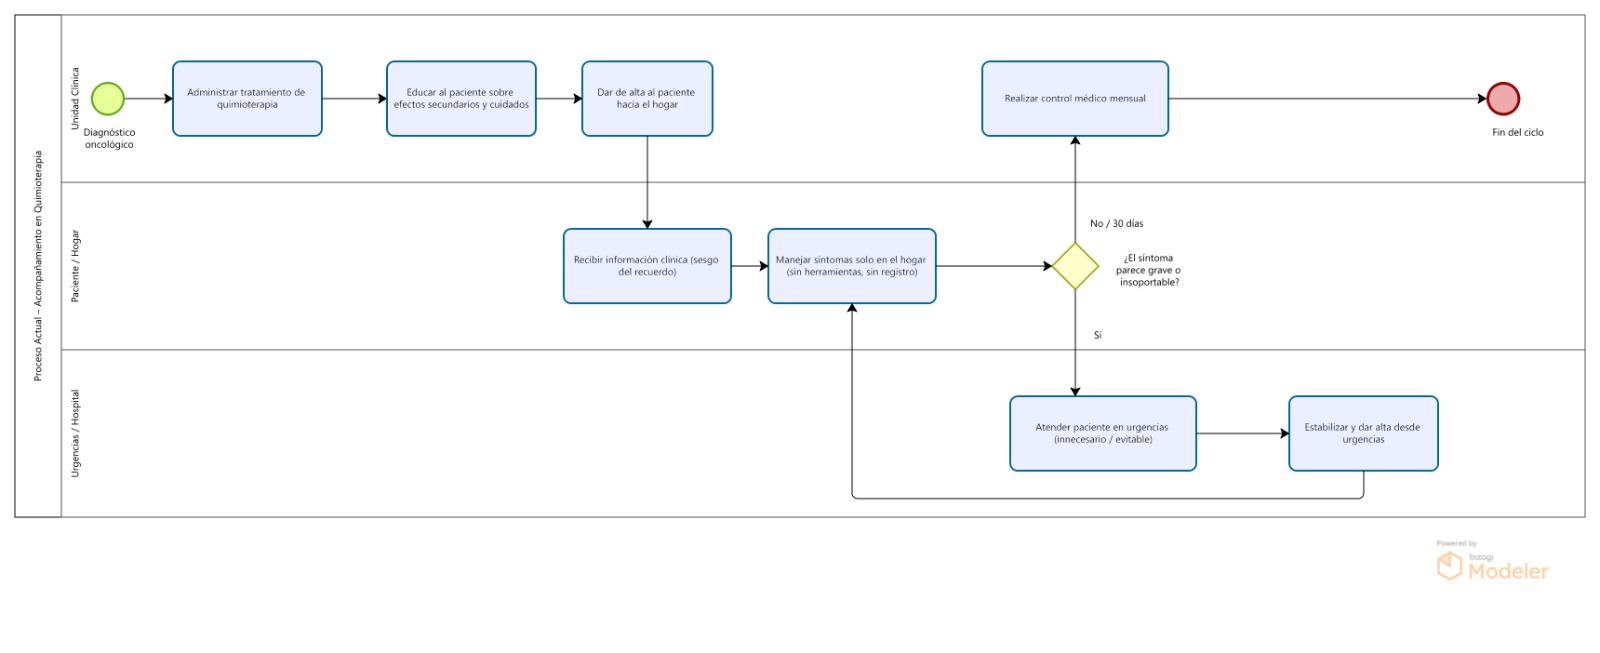
\includegraphics[
    width=1.1\paperwidth,
    height=1.1\paperheight,
    keepaspectratio
]{imagenes/bpmn_oncologia.png}

\captionof{figure}{Proceso de negocio “Acompañamiento en Oncología”}
\label{fig:BPMN Acompanamiento}
\vspace*{\fill}

\end{landscape}

\noindent
\textbf{BPMN 1 – Proceso actual de acompañamiento Oncológico (Figura \ref{fig:BPMN Acompanamiento})}

\noindent
El modelado del proceso de negocio evidenció el flujo operativo mediante el cual se ejecutaba el seguimiento de los pacientes en la Unidad de Quimioterapia del HCHM:

\noindent
El proceso se iniciaba al concluir la infusión citostática en la sala de quimioterapia. El personal de enfermería entregaba indicaciones verbales y folletos impresos con recomendaciones generales de autocuidado. A partir de ese momento, el paciente regresaba a su domicilio, asumiendo de manera autónoma la vigilancia y el registro de sus síntomas durante el período inter-ciclo.

\noindent
Ante la manifestación de toxicidades severas o alzas térmicas, el flujo dependía exclusivamente de la iniciativa del paciente o de su red de apoyo para trasladarse espontáneamente al Servicio de Urgencia del hospital o comunicarse telefónicamente. Al ingresar a la urgencia, el paciente se sometía al triage general sin disponer de un historial estructurado ni registro evolutivo de los parámetros fisiológicos previos, lo que demoraba la categorización médica y la identificación oportuna del nadir hematológico \parencite{minsal2022plancancer, entrevistaHCHM2026}.

\vspace{0.7cm}

\subsection*{Problemas detectados}
A partir de la triangulación entre la observación en terreno, las entrevistas semiestructuradas con el personal clínico del HCHM \parencite{entrevistaHCHM2026} y la revisión del Plan Nacional de Cáncer \parencite{minsal2022plancancer}, se consolidaron los siguientes problemas estructurales del área de estudio:

\begin{enumerate}
    \item \textbf{Latencia crítica en la identificación de toxicidades agudas:} La ausencia de un registro diario sistemático generó que complicaciones graves (neutropenia febril, deshidratación severa) fueran detectadas tardíamente, aumentando los ingresos de urgencia en estados clínicos deteriorados \parencite{minsal2022plancancer, entrevistaHCHM2026}.
    \item \textbf{Inoperatividad de soluciones dependientes de conectividad en red rural:} Debido a la alta dispersión y ruralidad en la Región de Ñuble, los sistemas basados exclusivamente en servicios en la nube quedaban inoperativos en zonas sin cobertura celular, impidiendo la emisión oportuna de alertas de riesgo en el hogar del paciente \parencite{ine2024censo, minsal2022plancancer}.
    \item \textbf{Ausencia de un motor de triaje determinista perimetral (\textit{edge}):} El entorno clínico no contaba con una solución móvil capaz de procesar signos vitales y síntomas de forma local e independiente de la red, imposibilitando la entrega de clasificaciones de gravedad inmediatas ante emergencias oncológicas.
    \item \textbf{Barrera de usabilidad en pacientes con fatiga y sobrecarga cognitiva:} Las herramientas digitales convencionales resultaban inadecuadas para pacientes sometidos a quimioterapia que presentaban cuadros de fatiga extrema o deterioro cognitivo leve transitorio, exigiendo una arquitectura de información simplificada y restringida a un máximo de tres pasos de interacción por flujo \parencite{entrevistaHCHM2026}.
    \item \textbf{Inexistencia de reportabilidad clínica estructurada:} La sobrecarga asistencial del equipo médico impedía la revisión manual de historiales extensos, haciendo necesaria una herramienta que consolidara y priorizara exclusivamente las variables fuera de rango clínico para optimizar la toma de decisiones en los controles de ciclo \parencite{entrevistaHCHM2026}.
\end{enumerate}